\chapter{弯曲内力}
\section{弯曲的概念}
\begin{definition}
    以弯曲形变为主的杆件习惯上称为梁。
\end{definition}

\begin{definition}
    当作用于杆件上的所有外力都在纵向对称面内时，弯曲形变后的轴线将是位于这个对称面内的一条曲线，我们称这种弯曲为对称弯曲。
\end{definition}

\section{受弯杆件的简化}
为了方便我们对弯曲杆件内力进行计算，我们对梁进行简化，得出计算简图。我们将重点讨论支座和载荷的简化。

\subsection{支座的几种基本形式}
\begin{itemize}
    \item 固定铰支座
    \item 可动铰支座
    \item 固定端支座
\end{itemize}
\begin{figure}[htbp]
  \centering
  % 子图1
  \begin{subfigure}{0.31\textwidth}
    \centering
    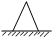
\includegraphics[width=0.8\linewidth]{Figure/固定铰支座.png}
    \caption{固定铰支座}
  \end{subfigure}
  \hfill
  % 子图2
  \begin{subfigure}{0.31\textwidth}
    \centering
    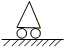
\includegraphics[width=0.8\linewidth]{Figure/可动铰支座.png}
    \caption{可动铰支座}
  \end{subfigure}
  \hfill
  % 子图3
  \begin{subfigure}{0.31\textwidth}
    \centering
    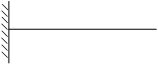
\includegraphics[width=0.8\linewidth]{Figure/固定端支座.png}
    \caption{固定端支座}
  \end{subfigure}
  \caption{支座示意图}
\end{figure}

\subsection{静定梁的几种基本形式}
\begin{itemize}
  \item 简支梁
  \item 外伸梁
  \item  梁
\end{itemize}



